\documentclass[a4paper, 12pt, onecolumn, openright, oneside]{report}

\usepackage{setspace} 
\usepackage[ansinew]{inputenc} 
\usepackage[T1]{fontenc} 
\usepackage[francais]{babel} 
\usepackage{color}
\usepackage{enumitem}
\usepackage{graphicx}
\usepackage{fancybox}
\usepackage{color}
\usepackage{geometry}
\usepackage{comment}
\usepackage{lipsum}% generates filler text
% ajoute (entre autre) la bibliographie dans la table des matieres 
\usepackage[french]{minitoc}
\usepackage[nottoc]{tocbibind}
\definecolor{rouge}{RGB}{255,112,119}
\definecolor{rouge-clair}{RGB}{255,163,168}
\definecolor{rouge-tres-clair}{RGB}{255,217,219}

\title{Rapport de stage}
\author{\textsc{Thibault} - \textsc{Gauthier}}
\date{Mise � jour  le \today}

\begin{document}
   \maketitle
   \chapter*{Remerciements}
\begin{flushright}
Je tiens à remercier toutes les personnes qui ont contribué au bon déroulement de mon stage.
\\En premier lieu Monsieur \textsc{Patrick Veillon}, Madame \textsc{Anne-Sophie Lescop} ainsi que l'entreprise Capgemini
qui m'ont donné l'opportunité et accordé leur confiance pour réaliser mon stage de fin d'études.
\\Je remercie également Monsieur \textsc{Jérome le Dorze}, Monsieur \textsc{Gaëtan Vieau} et toute l'équipe du projet Geofibre (\textsc{Omar, Olivier, Xavier, Jalal, Gaël, Sébastien, Damien, Taher}) pour leur aide et leurs conseils tout au long du stage.
\\Pour finir, je tiens à manifester ma gratitude à Messieurs \textsc{Mickaël Foursov, Charles Queguiner, François Poulet et Didier Certain} ainsi qu'à l'ensemble des enseignants pour le bon déroulement de ces trois années du cursus MIAGE.
\end{flushright}

   \tableofcontents
   \chapter*{Introduction}
\addstarredchapter{Introduction}
La fin du master \textit{MIAGE} se concrétise par la réalisation d’un stage en entreprise d’une durée de 6 mois.
\\J’ai choisi de réaliser ce stage au sein de l’entreprise \textsc{Capgemini} du 9 mars au 21 août 2015,
dans le centre de services \textit{TMA OSS}\footnote{Tierce Maintenant Applicative des applications orientés réseau d'Orange} à Rennes.
\\Mon choix s’est porté sur ce stage pour plusieurs raisons.
 Tout d’abord la présentation du sujet m'a séduit, le projet \textit{Geofibre} m'a beaucoup plu.
 Ensuite, mes différentes expériences de stage ayant jusqu’alors été réalisées en
autonomie ou en binôme, je souhaitais intégrer une équipe de travail déjà en place.
\\Pour finir, je n'ai encore jamais travaillé dans une \textit{ESN}\footnote{Entreprise de services du numérique}, c'était l'occasion de se
faire une opinion.
\\\\
Dans un premier temps je présenterai le contexte du stage, l'entreprise d'accueil et le projet sur lequel j'ai travaillé.
Puis, dans un second temps je présenterai le stage en lui-même.

   
   \part{Environnement}
   \chapter{La société Capgemini}
\subsection*{Introduction}
Capgemini est une ESN\footnote{Entreprise de services du numérique} multinationale spécialisée dans le génie logiciel.
\\Elle a été créee le 1er Octobre 1967 à Grenoble par Monsieur \textsc{Serge Kampf} et elle est actuellement dirigée par  Monsieur \textsc{Paul Hermelin}.\\
En France, elle est la première dans son domaine en terme de chiffre d'affaire. \'A l'internationale, elle figure parmi les cinq premiers.
\\Capgemini est notamment côtée en bourse au CAC40.
\\\\
\begin{figure}[h]
  \captionbox{Monsieur Serge KAMPF\label{fig:dummy}}{
    
\includegraphics[width=4cm]{images/sergekampf.png}
  }
  \captionbox{Monsieur Paul HERMELIN\label{fig:dummy}}{
    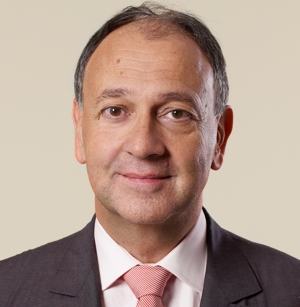
\includegraphics[width=4cm]{images/paulhermelin.png}
  }
  \captionbox{Logo de Capgemini\label{fig:dummy}}{
    
\includegraphics[width=5cm]{images/logo_capgemini.png}
  }
\end{figure}

\newpage
\section{Fiche d'identité}
\begin{description}
  \item[Raison sociale] : Capgemini
  \item[Année de création] : 1967
  \item[Fondateur] : Serge Kampf
  \item[Forme juridique] : Société anonyme à conseil d'administration
  \item[Siège social] : Paris
  \item[Directeur Général] : Paul Hermelin
  \item[Présence internationale] : 40 pays
  \item[Effectif en 2014] : 145 000
  \item[Chiffre d'affaire en 2014] : 10,6 milliards d'euros
\end{description}
\begin{figure}[h]
  \captionbox{Chiffre d'affaire par pays (2014)\label{fig:dummy}}{
    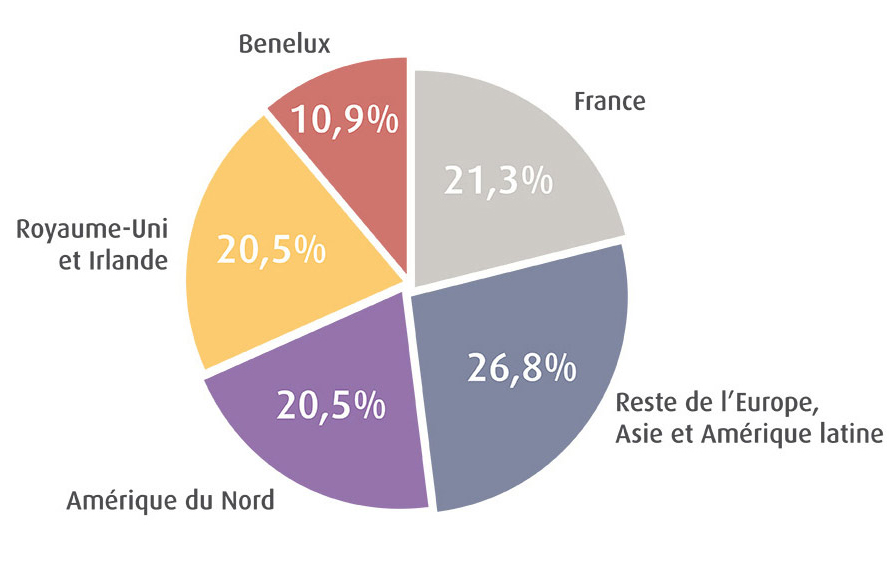
\includegraphics[width=15cm]{images/capays.png}
  }
\end{figure}
\newpage
\section{Métiers et activités}
\subsection{Secteurs d'activités}
Capgemini est spécialisé dans 6 secteurs d'activités :
\\
\begin{enumerate}
\item \textbf{Télécom, Média et \textit{Entertainment}}
\item \textbf{\'Energie, \textit{utilities} et chimie.}
\item \textbf{Industrie manufacturière et pharmaceutique}
\item \textbf{Services financiers}
\item \textbf{Grande consommation, distribution, transport et logistique}
\item \textbf{Services publics}\\
\end{enumerate}
\begin{figure}[h]
  \captionbox{Chiffre d'affaire par secteur (2014)\label{fig:dummy}}{
    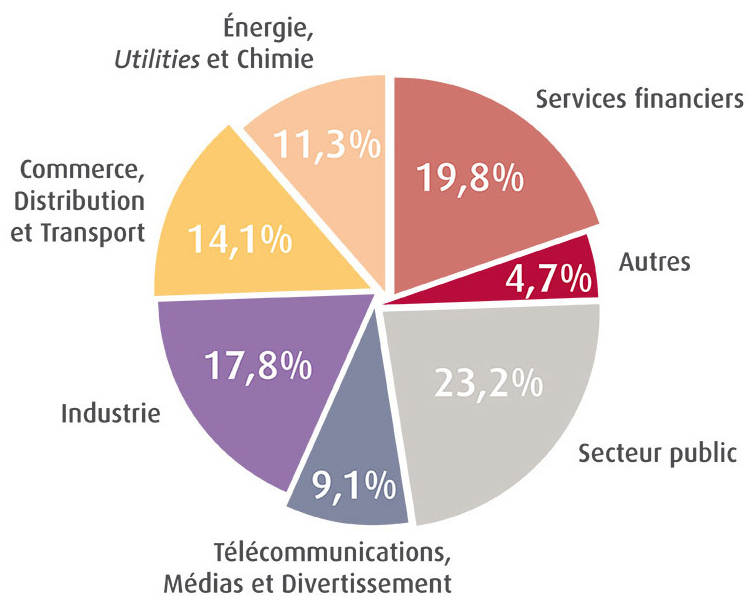
\includegraphics[width=12cm]{images/casecteur.png}
  }
\end{figure}
\newpage
\subsection{Métiers}
Capgemini travail dans 4 métiers principaux :
\\
\begin{enumerate}
\item \textbf{Le conseil en management (Capgemini Consulting)} a pour mission de contribuer, au travers d’actions telles que la transformation de l’activité ou la redéfinition de grandes fonctions, à l’amélioration des performances économiques des entreprises, grâce à une connaissance approfondie de leurs métiers et de leurs processus.
\item \textbf{L'intégration de systèmes et le développement d'applications} fait appel à la capacité de concevoir et d’intégrer des solutions, d’exploiter les innovations et de transformer l’environnement technologique.
\item \textbf{L’infogérance (Outsourcing Services - OS)} se concrétise par une prise en charge totale ou partielle de la gestion des ressources informatiques du client. Le Groupe a développé une gamme de services de gestion de systèmes informatiques, d’optimisation des processus métiers et de flexibilité des coûts de structures afin d’améliorer le rapport coût/performance.
\item \textbf{L'assistance technique et services de proximité (Sogeti)} ) sont implantés géographiquement au plus près des décideurs techniques locaux des grandes entreprises, visant à soutenir les capacités internes des directions informatiques en leur proposant dans des délais les plus brefs les meilleurs spécialistes.
\end{enumerate}
\begin{figure}[h]
  \captionbox{Chiffre d'affaire par metiers (2014)\label{fig:dummy}}{
    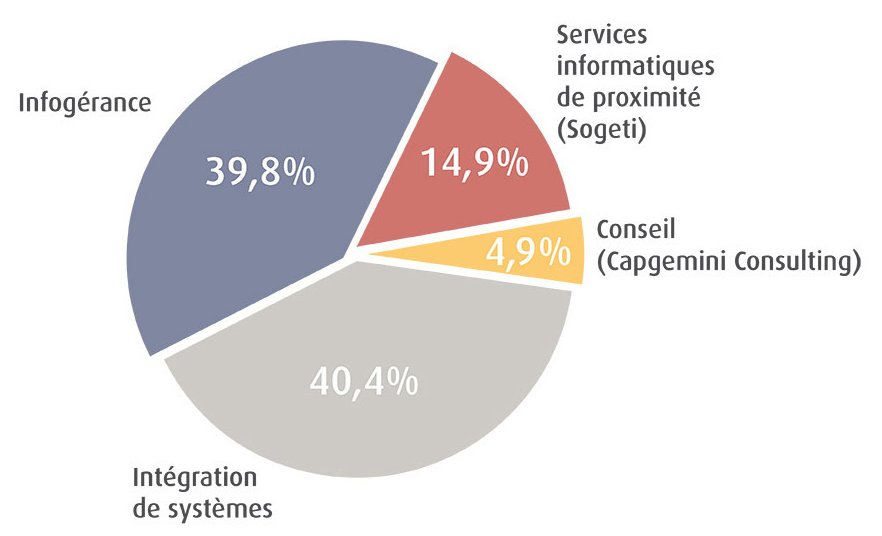
\includegraphics[width=13cm]{images/cametier.png}
  }
\end{figure}

    \chapter{Le center de service TMA OSS}
    \chapter{Le domaine de comp�tence SIG}
   \chapter{Le projet Géofibre}
\section{Objet}
Le projet \textit{Geofibre} a pour objet de fournir une application de \textit{SIG} pour \textsc{Orange} dans le domaine du \textit{FTTH}\footnote{Fiber To The Home : C'est le réseau trés haut débit de fibre optique pour les clients résidentiels.}.\\
L'application se présente sous la forme d'une page Web permettant de gérer et concevoir des données descriptives du réseau \textit{FTTH} en France Métropolitaine (\textit{et depuis peu dans les départements d'Outre-Mer}), en temps réel avec plusieurs utilisateurs connectés simultanément.\\
Cette application est principalement destinée aux chargés d'affaire et sous-traitant \textit{FTTH}.\\
Elle a pour mission, par exemple, de faire évoluer le réseau en permettant la conception sur l'application pour ensuite l'imprimer et l'installer sur le terrain ou par exemple avoir une vision globale des installations sur une commune.\\
En matière de charge, elle comptabilise en 2015 jusqu'à \textbf{1150 utilisateurs simultanés}.\\
Techniquement \textit{Geofibre} est basé sur le progiciel \textit{ArcGIS} de l'éditeur \textsc{ESRI}.

\newpage
\section{Historique}
Le lancement du projet a eu lieu en 2010. Jusqu'en 2012 le projet s'est développé dans les locaux du client dans la ville de Lannion suivant la méthode de gestion de projets \textit{AGILE}.\\
Les employés de la société \textsc{Capgemini} étaient à cette époque présents dans les locaux du client pour travailler en tant qu'assistants techniques.
Par la suite le développement du projet s'est réalisé dans les locaux de \textsc{Capgemini}, au \textit{Spirea} à Rennes.\\\\
Depuis ses débuts \textit{Geofibre} a évolué de manière significative. \'A l'heure actuelle le projet est à sa 7ème version mineure(cf.\ref{versionning}) et des évolutions sont prévues, d'autant que le gouvernement Français souhaite développer la fibre optique sur l'ensemble du territoire Français.

\section{Illustration}
\begin{figure}[h]
	\captionbox{Capture d'écran du projet Geofibre\label{fig:dummy}}{
		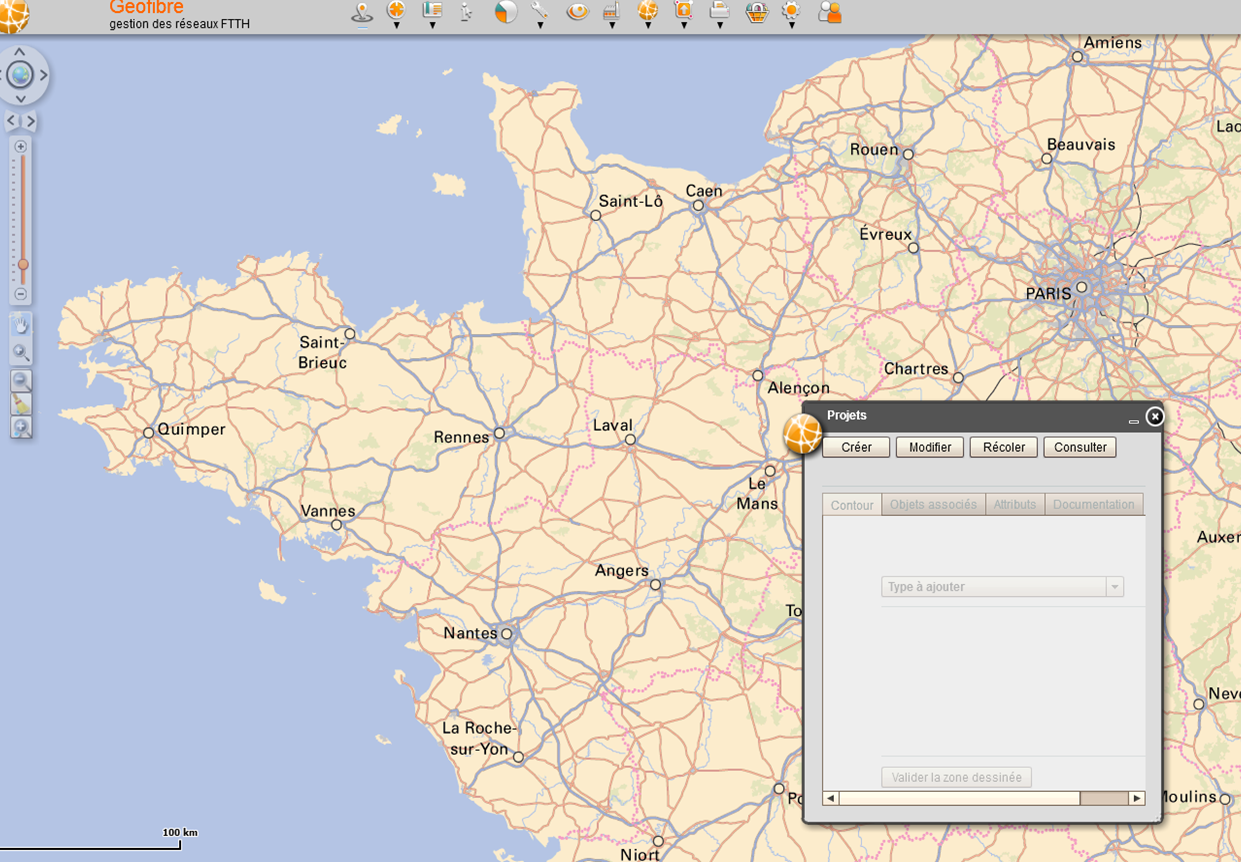
\includegraphics[width=16cm]{images/shotgeofibre.png}
	}
\end{figure}

   
   \part{Travaux r�alis�}
   \chapter{Travaux sur le projet Geofibre}

\section{Mont�e en comp�tence}
\subsection{Outils et technologies}
\subsection{Architecture du projet}
\subsection{Architecture technique}
\subsection{Architecture logicielle}
\subsection{Lexique SIG}
\subsection{Lexique FTTH}
\subsection{Processus de d�veloppement Capgemini}

\section{D�veloppements pour la version G1R6}
\subsection{Externalisation des param�tres}

\section{Tests la version G1R6}
\subsection{Tests d'int�gration des DOM}
\subsection{Tests de non-r�gression de la France M�tropolitaine}

\section{Correction d'anomalies �ligibles pour la version G1R7}
\subsection{Exemple d'une correction}
   \chapter{E-learning}
   \chapter*{Résumé}
\addstarredchapter{Résumé} 

   \chapter*{Abstract}
\addstarredchapter{Abstract}

My \textit{Master 2 MIAGE} internship was carried out within the company \textsc{Capgemini} at Rennes during six month.
\\\\
Within the service \textit{TMA OSS} I participated in the development and maintenance on \textit{Geofibre} application.
This application of \textit{GIS} enables business managers, via a \textit{web GUI}, to manage and develop the domestic \textit{FTTH} network in metropolitan France.
\\\\
My role was to provide the support to the development team for the integration of a new version of the application
to manage the \textit{FTTH} network of Overseas Departments ( French Guyana, Guadeloupe , Martinique and Réunion) .
Then, during the specification phase of the next release I spent to correct severals defects noted by the client.
Finally I participated in the development and integration of the latest version of the application that makes the management of new operators data.

   \chapter*{Conclusion}
\addstarredchapter{Conclusion}

Pour commencer le projet Geofibre est très intéressant de bout en bout et pour commencer m'a permis de découvrir le monde du SIG et du FTTH.
\\Techniquement j'ai pu découvrir le langage ActionScript et le framework Flex avec la programmation évenementiel même si c'est une technologie de moins en moins utilisée.
 \\ J'ai aussi pu découvrir le fonctionnement et l'utilité du progiciel ArcGIS.
 \\Aussi j'ai appris beaucoup de petites techniques de développement et de débuguage, notamment sur l'IDE Eclipse/FlashBuilder et en PostgreSQL.
\\\\Professionnellement cela m'a permis d'enrichir mon expérience et de mieux comprendre les différentes phases de déroulement d'un projet, ainsi que le développement et la méthodologie de travail dans un contexte industriel.
\\\\En ce qui concerne mon apport pour l'entreprise \textsc{Capgemini}, les évolutions développés et testés pour la version G1R6 ont été livrées à Orange et vont être utilisé en production.
\\\\Le stage m'a beaucoup apporté. J'ai travaillé avec une jeune équipe, qualifiée et compétente qui m'ont énormément aidé. J'ai pu apprendre, observer et acquérir de nouvelles compétences mais aussi apporter le fruit de mes années d'études au projet.

   \appendix 
      \chapter{Bibliographie / Webographie}
\begin{description}
\item{[1]} [..]
\item{[2]} [..]
\item{[3]} [..]
\end{description} 
      \chapter{Carnet de bord des travaux r�alis�s par semaine}
\begin{enumerate}[label= Semaine \no\textbf{\arabic*.},itemsep=20pt]
\setcounter{enumi}{10}

\item \textbf{Visite, pr�sentation et rencontre} avec les �quipes de la ferme d'applications \textsc{TMA OSS\footnote{Tierce Maintenant Applicative des applications orient�s r�seau d'Orange}}. Explication de l'activit� par le chef de service \textsc{Arnaud Bellina}.
\newline Visite, pr�sentation et rencontre avec les diff�rents services du b�timent de Capgemini (Infirmerie, CE, Caf�taria, RH, Assistante) .
\newline \textbf{Installation de mon poste de travail} au sein de l'openspace de l'�quipe G�ofibre et int�gration supervis�e par le chef de groupe \textsc{Patrick Veillon} et la chef de projet \textsc{Anne-Sophie Lescop}.
\newline \textbf{Installation des logiciels} et \textbf{lecture} de la documentation ainsi que du code qui compose le projet G�ofibre �paul� par l'�quipe.

\item \textbf{Mont�e en comp�tence} g�n�rale sur l'application G�ofibre.
\item \textbf{D�veloppement de la version G1R6 Front (IHM Flex)} Externalisation des syst�mes de projection, emprise, �chelles, minimap

\item \textbf{D�veloppement de la version G1R6 Back (Serveur, Toolbox)} V�rification de la gestion de la projection

\item \textbf{D�veloppement de la version G1R6 Back (Serveur, Toolbox)} Aiguillage servlet
\newline \textbf{D�veloppement de la version G1R6 Back (Serveur, Toolbox)} Impact code appelant

\item \textbf{Tests d'int�gration de la version G1R6 sur la R�union}
\begin{enumerate}[label = Tests \no\arabic*.,align=left]
\item \emph{\colorbox{rouge}{P1}} - Gestion infrastructure - Recalage GC
\item \emph{\colorbox{rouge}{P1}} - Gestion infrastructure - Zone de recalage
\item \emph{\colorbox{rouge-clair}{P2}} - Exploitation - Import RCV (R�f�renciel Commune Voies)
\item \emph{\colorbox{rouge-clair}{P2}} - Localisation adresse
\item \emph{\colorbox{rouge-tres-clair}{P3}} - Purge des fichiers (multi instance)
\end{enumerate}

\item \textbf{Tests d'int�gration de la version G1R6 sur la Guyane}
\begin{enumerate}[label = Tests \no\arabic*.,align=left]
\item  \emph{\colorbox{rouge}{P1}} - Gestion FTTH - C�bles
\item \emph{\colorbox{rouge}{P1}} - Gestion FTTH - Parcours
\item\emph{\colorbox{rouge}{P1}} -  Gestion FTTH - Zone de travail
\item \emph{\colorbox{rouge}{P1}} - Gestion infrastructure - Itin�raires GC
\item \emph{\colorbox{rouge}{P1}} - Gestion infrastructure - Site supports
\item \emph{\colorbox{rouge-tres-clair}{P3}} - Filtrage
\item \emph{\colorbox{rouge-tres-clair}{P3}} - Gestion des droits
\item \emph{\colorbox{rouge-tres-clair}{P3}} - G�osignets
\item \emph{\colorbox{rouge-tres-clair}{P3}} - Outil de mesure
\item \emph{\colorbox{rouge-tres-clair}{P3}} - Sauvegarde du contexte
\item \emph{\colorbox{rouge-tres-clair}{P3}} - Table des mati�res
\end{enumerate}

\item \textbf{Tests d'int�gration de la version G1R6 sur la Guadeloupe}
\begin{enumerate}[label = Tests \no\arabic*.,align=left]
\item \emph{\colorbox{rouge}{P1}} - Gestion infrastructure - Site supports
\item \emph{\colorbox{rouge}{P1}} - Exports - Dossier OPGC - Base arri�re de PM
\item \emph{\colorbox{rouge-clair}{P2}} - M�j adresse des immeubles depuis optimum
\item \emph{\colorbox{rouge-clair}{P2}} - Exploitation - majBatchData
\item \emph{\colorbox{rouge-clair}{P2}} - Statistiques
\item \emph{\colorbox{rouge-tres-clair}{P3}} - Filtrage
\item \emph{\colorbox{rouge-tres-clair}{P3}} - Gestion des droits
\item \emph{\colorbox{rouge-tres-clair}{P3}} - G�osignets
\item \emph{\colorbox{rouge-tres-clair}{P3}} - Localisation objet m�tier
\end{enumerate}

\item \textbf{Tests d'int�gration de la version G1R6 sur la Martinique}
\begin{enumerate}[label = Tests \no\arabic*.,align=left]
\item  \emph{\colorbox{rouge}{P1}} - Gestion FTTH - C�bles
\item \emph{\colorbox{rouge}{P1}} - Gestion FTTH - Parcours
\item \emph{\colorbox{rouge}{P1}} - Gestion infrastructure - Itin�raires GC
\item \emph{\colorbox{rouge}{P1}} - Gestion FTTH - Projets
\item \emph{\colorbox{rouge}{P1}} - Gestion FTTH - Sch�ma directeur
\item \emph{\colorbox{rouge}{P1}} - Gestion FTTH - R�gles d'ingienerie
\item \emph{\colorbox{rouge}{P1}} - D�calages horaires
\item \emph{\colorbox{rouge-clair}{P2}} - Statistiques
\item \emph{\colorbox{rouge-tres-clair}{P3}} - Filtrage
\item \emph{\colorbox{rouge-tres-clair}{P3}} - Gestion des droits
\item \emph{\colorbox{rouge-tres-clair}{P3}} - Outil de mesure
\item \emph{\colorbox{rouge-tres-clair}{P3}} - Sauvegarde du contexte
\end{enumerate}
\textbf{Prise en main du logiciel ArcMap de la suite ArcGis.}
\item \textbf{Tests de non-regression de la version G1R6 sur la France m�tropolitaine}
\begin{enumerate}[label = Tests \no\arabic*.,align=left]
\item  \emph{\colorbox{rouge}{P1}} - Impression
\end{enumerate}
\textbf{Anomalie relev� sur les zones d'�gilibilit�s}
\newline
\textbf{Formation E-Learning}
\begin{enumerate}[label = Formation \no\arabic*.,align=left]
	\item \textit{Utiliser efficacement l'email et la messagerie isntantanee}
	\item \textit{Utiliser le Brown Paper}
	\item \textit{Utiliser du Portail MyLearning}
\end{enumerate}
\item \textbf{Tests de non-regression de la version G1R6 sur la France m�tropolitaine}
\begin{enumerate}[start = 2,label = Tests \no\arabic*.,align=left]
\item  \emph{\colorbox{rouge}{P1}} - Gestion FTTH - C�bles
\item  \emph{\colorbox{rouge}{P1}} - Gestion FTTH - R�gles d'ingienerie
\end{enumerate}
\textbf{Formation E-Learning}
\begin{enumerate}[label = Formation \no\arabic*.,align=left]
	\item \textit{Les fondamentaux du test logiciel}
\end{enumerate}

\newpage
\item \textbf{Pr�sentation du d�roulement de mon stage} Collecte d'informations sur le centre de service  \textsc{TMA OSS\footnote{Tierce Maintenant Applicative des applications orient�s r�seau d'Orange}} et le domaine de comp�tence \textsc{SIG\footnote{Syst�me d'Information G�ographique}} auquel se rattache le projet G�ofibre sur lequel j'effectue mon stage. Cr�ation d'un diaporama pour cette pr�sentation. R�alisation de la pr�sentation avec une dizaine de stagiaires, la responsable DRH et les diff�rents chefs de projets.
\newline
\textbf{Formation E-Learning}
\begin{enumerate}[label = Formation \no\arabic*.,align=left]
	\item \textit{La politique anti-corruption du groupe}
	\item \textit{Les lois de la concurrence}
	\item \textit{Les normes �cologique du groupe}
	\item \textit{Le code �thique dans la relation client}
\end{enumerate}
\item
\textbf{Correction d'anomalies hors-garantie �ligibles pour la version G1R7}
\textbf{Redaction et passage des \textsc{TU\footnote{Tests Unitaires}} relatifs aux corrections}
\begin{enumerate}[label = Correction \no\arabic*.,align=left]
	\item \textit{Repositionnement d'immeubles en masse} - Perte de la s�lection d'immeubles apr�s avoir annul� une fen�tre de choix d'immeuble.
	\item \textit{Repositionnement d'immeubles s�quentiel} - Perte de la s�lection d'immeubles apr�s avoir annul� une fen�tre de choix d'immeuble.
	\item \textit{Visu Shape} - Message d'erreur a tord "Le nombre maximum de fichiers visualis�s simultan�ment est de 5".
\end{enumerate}
\textbf{Formation E-Learning}
\begin{enumerate}[label = Formation \no\arabic*.,align=left]
	\item \textit{Communiquer avec assurance}
	\item \textit{Entretenir de bons rapports avec le client}
\end{enumerate}

\item
\textbf{Correction d'anomalies hors-garantie �ligibles pour la version G1R7}
\textbf{Redaction et passage des \textsc{TU\footnote{Tests Unitaires}} relatifs aux corrections}
\begin{enumerate}[label = Correction \no\arabic*.,align=left]
	\item \textit{Sites supports} - Perte d'information du champs gestionnaire lors de la duplication si celui-ci a la valeur "39" en production. (en attente d'informations d'Orange)
	\item \textit{C�bles, alv�oles} -  Suppression des donn�es d'alv�oles non homog�ne (en attente d'informations d'Orange)
\end{enumerate}
\textbf{Formation E-Learning}
\begin{enumerate}[label = Formation \no\arabic*.,align=left]
	\item \textit{El�ments d�une �quipe soud�e}
	\item \textit{Etablir des relations de confiance}
	\item \textit{Etre un membre efficace au sein d�une �quipe}
\end{enumerate}
\textbf{Breizhcamp}
\item
\textbf{Correction d'anomalies hors-garantie �ligibles pour la version G1R7}
\textbf{Redaction et passage des \textsc{TU\footnote{Tests Unitaires}} relatifs aux corrections}
\begin{enumerate}[label = Correction \no\arabic*.,align=left]
	\item \textit{Connexion} -  Geofibre ne g�re pas la casse du cu\_id d'un utilisateur.
	\item \textit{Impression Libre et Casage} - Perte de la valeur par d�faut du champ R�solution
\end{enumerate}
\textbf{Formation E-Learning}
\begin{enumerate}[label = Formation \no\arabic*.,align=left]
	\item \textit{Limitation des voleurs de temps}
	\item \textit{Contr�ler son stress}
	\item \textit{Planifier et hierarchiser son temps}
\end{enumerate}
\item
\textbf{Support � Taher qui viens d'arriver sur le projet}\\
\textbf{Correction d'anomalies hors-garantie �ligibles pour la version G1R7}\\
\textbf{Redaction et passage des \textsc{TU\footnote{Tests Unitaires}} relatifs aux corrections}\\
\begin{enumerate}[label = Correction \no\arabic*.,align=left]
	\item \emph{\colorbox{rouge}{majeure}} \textit{Flux cables} -  Echec de l'import sur pr�sence de point virgule , simple guillement ou double guillemet
\end{enumerate}
\textbf{D�tection de la version d'anomalie}\\
Certaines anomalies sont en garantie (versions G1R4, G1R5, G1R6) dans quel cas si le client les trouve il faudra les corriger.
D'autres sont hors-garantie (< G1R4) Dans ce cas il faut les annoncer aux clients et ils d�cident si ils veulent les corriger ou non.
\\
Pour cela il faut d�tecter ou est-ce que l'anomalie est situ�e dans le code et voir � quel moment les changements ont �t� commit� sur le gestionnaire de version SVN. En fonction de la date du commit ou du TAG
ont peut remonter au num�ro de version.
\begin{enumerate}[label = D�tection de la version d'anomalie \no\arabic*.,align=left]
	\item \textit{Points techniques} - Il est possible cr�er un PT avec une r�f�rence de plus de 25 caract�res
	\item \textit{Points techniques} - Import - Probl�me d'encodage dans les comptes rendus
\end{enumerate}
\textbf{Correction d'anomalies hors-garantie �ligibles pour la version G1R7}\\
\textbf{Redaction et passage des \textsc{TU\footnote{Tests Unitaires}} relatifs aux corrections}
\begin{enumerate}[label = Correction \no\arabic*.,align=left]
	\item \textit{Recalcul nombre d'EL} -majBatchData.ksh,KO si  la zone est � cheval sur deux communes [ksh, SQL, PostGIS]
\end{enumerate}
\textbf{Les sp�cifications de la version G1R7 ont �t� livr� et valid�. Les d�veloppements peuvent commencer !}
\item
\textbf{G1R7} Lecture assidu des sp�cifications\\
\textbf{G1R7} D�veloppement - [Site support] Ajout du champs d�ployeur en BDD\\
\textbf{Correction d'anomalies hors-garantie �ligibles pour la version G1R7}\\
\textbf{Redaction et passage des \textsc{TU\footnote{Tests Unitaires}} relatifs aux corrections}
\begin{enumerate}[label = Correction \no\arabic*.,align=left]
	\item \textit{Visu Shape} -sauvegarde dans le contexte utilisateur d'un shape non valide [IHM]
\end{enumerate}
\textbf{G1R7} D�veloppement - [Site support] Ajout du champs d�ployeur dans l'IHM\\
\item
\textbf{G1R7} D�veloppement - [Annexe C3A] Nouvelle gestion du diam�tre des parcours
\item
\item
\item
\item
\item
\item
\item
\item
\end{enumerate}

\end{document}